\documentclass[12pt]{article}

\usepackage[utf8]{inputenc}
\usepackage{graphicx}
\usepackage{float}
\usepackage{amsmath}
\usepackage{placeins}
\usepackage{gensymb}
\usepackage{caption}
\usepackage{subcaption}
\setcounter{section}{-1}


\usepackage[letterpaper,margin=0.75in]{geometry}
\graphicspath{images/}
\begin{document}
\begin{titlepage}
\begin{center}
% Upper part of the page
\vbox{}
\vbox{}
\vbox{}
\vbox{}
\vbox{}
\vbox{}
\vbox{}
\vbox{}
\vbox{}

\includegraphics[width=0.75\textwidth]{Images/ubc.png}\\[0.5cm]
\textrm{Martin Alejo}\\[0.5cm]
\catcode`#=12
\textrm{#75296665}\\[0.5cm]
\textrm{December 9, 2022}\\[0.5cm]
\textrm{Mini Project 4}\\[0.5cm]
\textrm{University of British Columbia}\\[0.5cm]
\textrm{Electrical and Computer Engineering}\\[0.5cm]
\textrm{ELEC 301}\\[0.5cm]
\textrm{Instructor: Nicolas Jaeger}\\[0.5cm]

\includegraphics[width=0.18\textwidth]{Images/Signature.png}\\[0.5cm]
\vbox{ }
\end{center}
\end{titlepage}
\pagebreak
\pagenumbering{roman}
\tableofcontents
\pagebreak
\listoffigures
\listoftables
\pagebreak
\pagenumbering{arabic}


\section{Introduction}
For this project, we will be using Multisim to simulate active filters and oscillators.
\section{Part A}
\subsubsection{Part 1}
For this part, we will be designing a 2nd order Butterworth low pass active filter using the UA741 operational amplifier. 
Here is the circuit that we will be using for this part:

\begin{figure}[H]
    \centering
    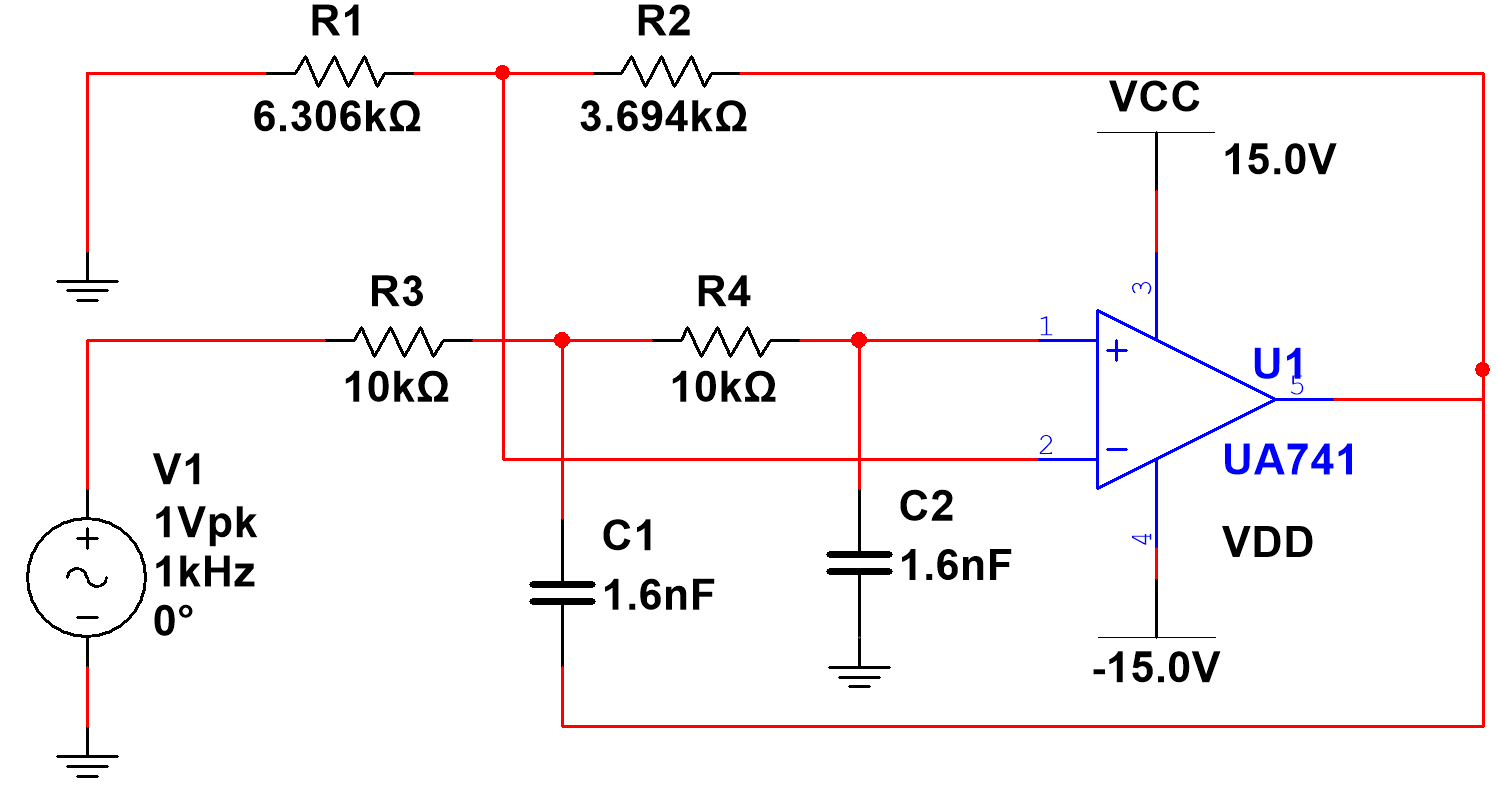
\includegraphics[height=0.2\textwidth]{Images/partAcircuit.png}\\
    \caption{Second Order Butterworth Filter}
    \label{fig:SecondOrderButterworthFilter}
\end{figure}

The calculations to find the resistance $R_1$,$R_2$ and capacitance C, we will be using the formulas from the class notes [1].  
The formulas can also be found from no. 1 in the Appendix. From the formulas, we can see that

\begin{center}
\boxed{R_1 = 6.306k \Omega, R_2 = 3.694k\Omega, C = 1.6nF, A_m = 1.59\frac{V}{V}}
\end{center}
Below is the phase and magnitude plot for our filter:

\begin{figure}[H]
    \centering
    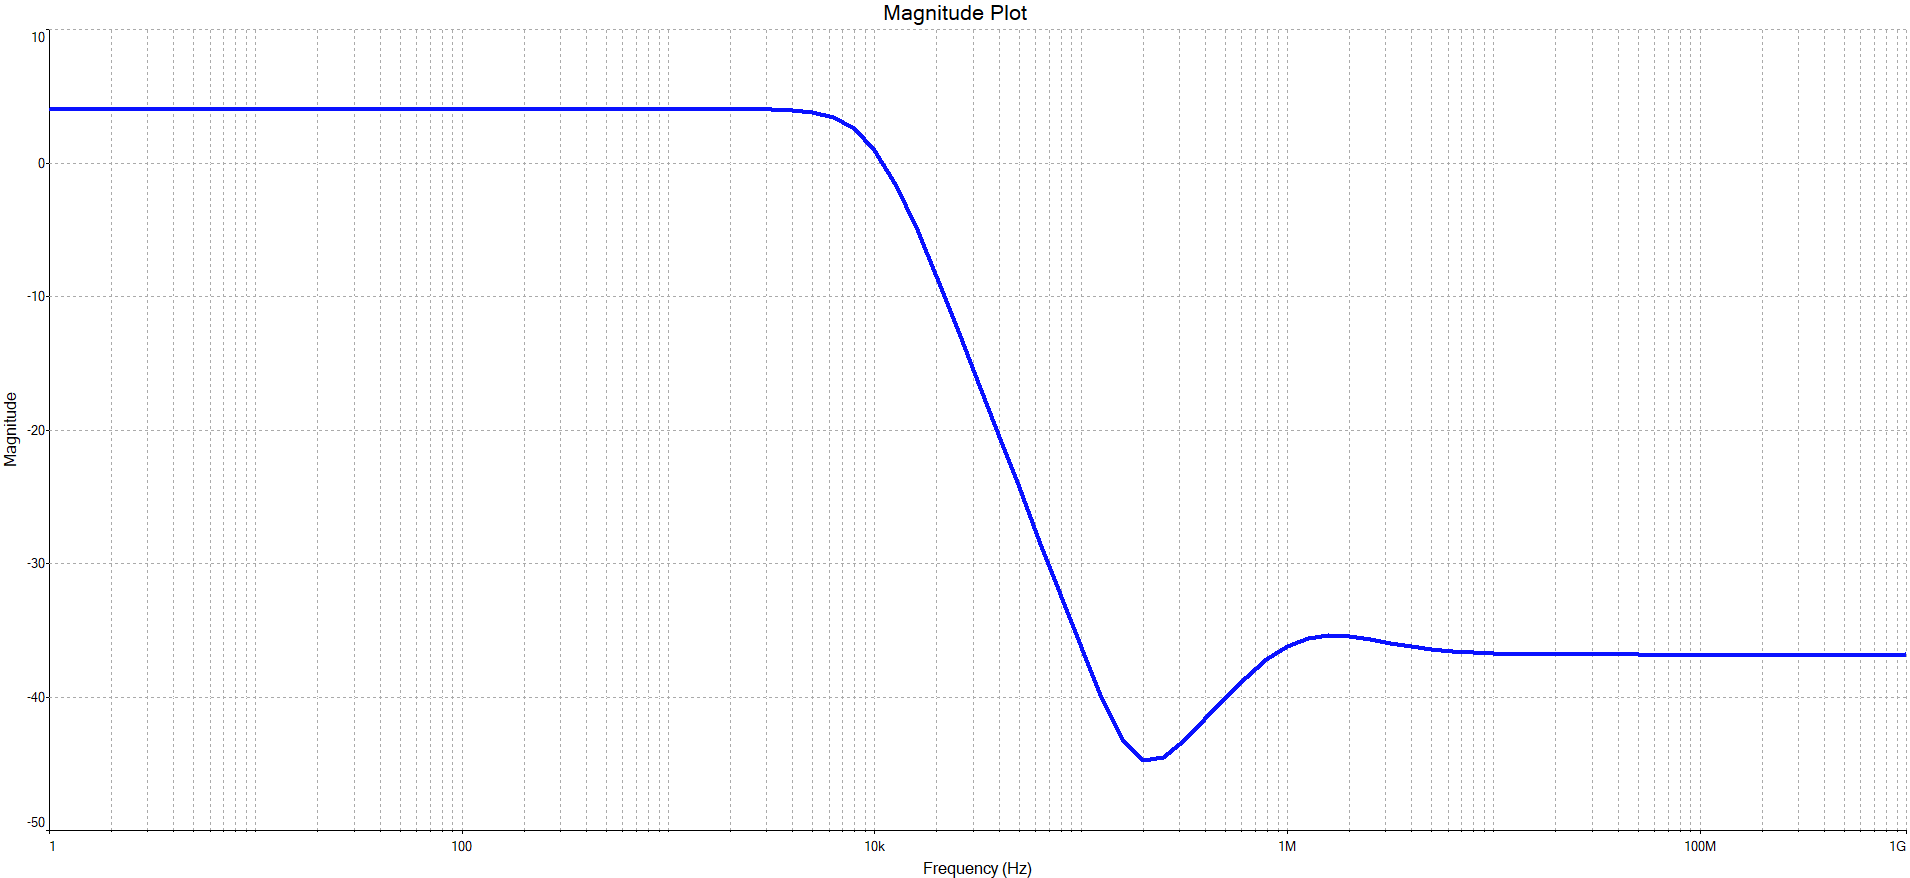
\includegraphics[height=0.4\textwidth]{Images/magnitude_plot.png}\\
    \caption{Bode Magnitude Plot}
    \label{fig:magntitudeplot}
\end{figure}


\begin{figure}[H]
    \centering
    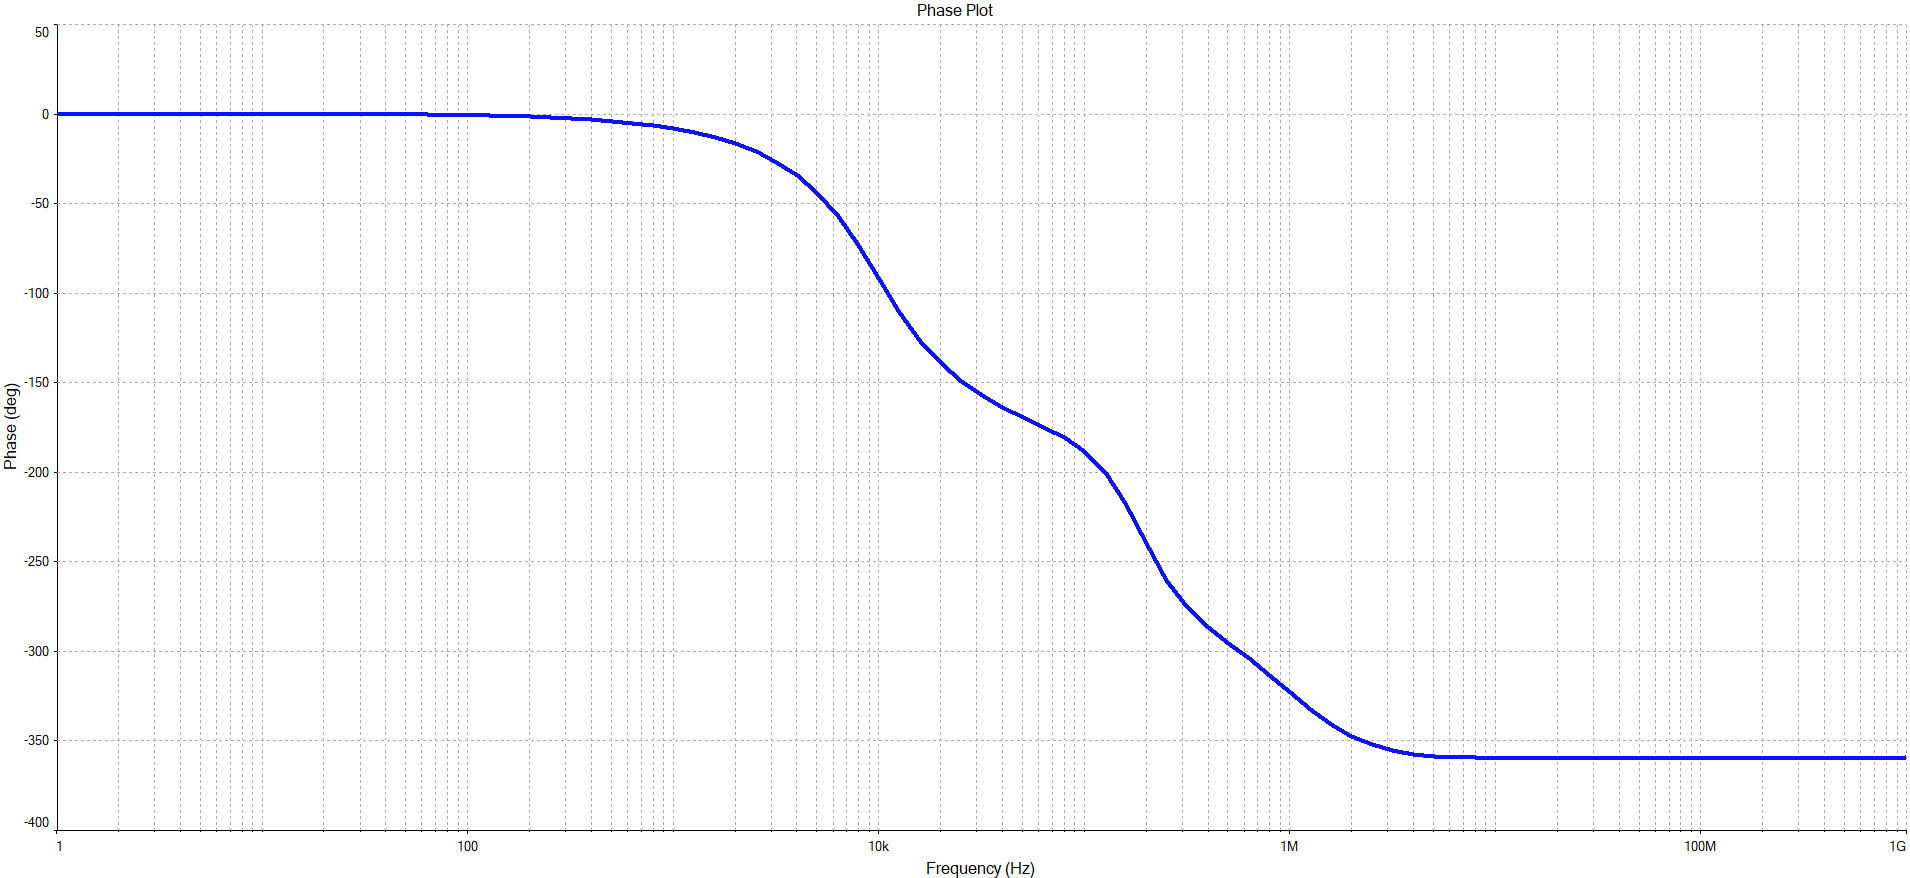
\includegraphics[height=0.4\textwidth]{Images/phase_plot.png}\\
    \caption{Bode Phase Plot}
    \label{fig:phaseplot}
\end{figure}


\subsubsection{Part 2}
For this part, we will be grounding the input, and measuring the output of the OpAmp.
To determine the value of $A_m$ when the circuit begins to oscillate, we need the transfer fucntion. The function is shown below,
where R = $10k\Omega$ and C is the value found previously:
\begin{flalign}
&H(s) = A_M\frac{\frac{1}{(RC)^2}}{s^2+s\frac{3-A_M}{RC}+\frac{1}{(RC)^2}}\nonumber
\end{flalign}
Changing the values of the resistances, we find that the oscillations occour when the resistor values are around$R_1=3k\Omega$ and $R_2 =
7k\Omega$.
The oscillation is shown below:
\begin{figure}[H]
    \centering
    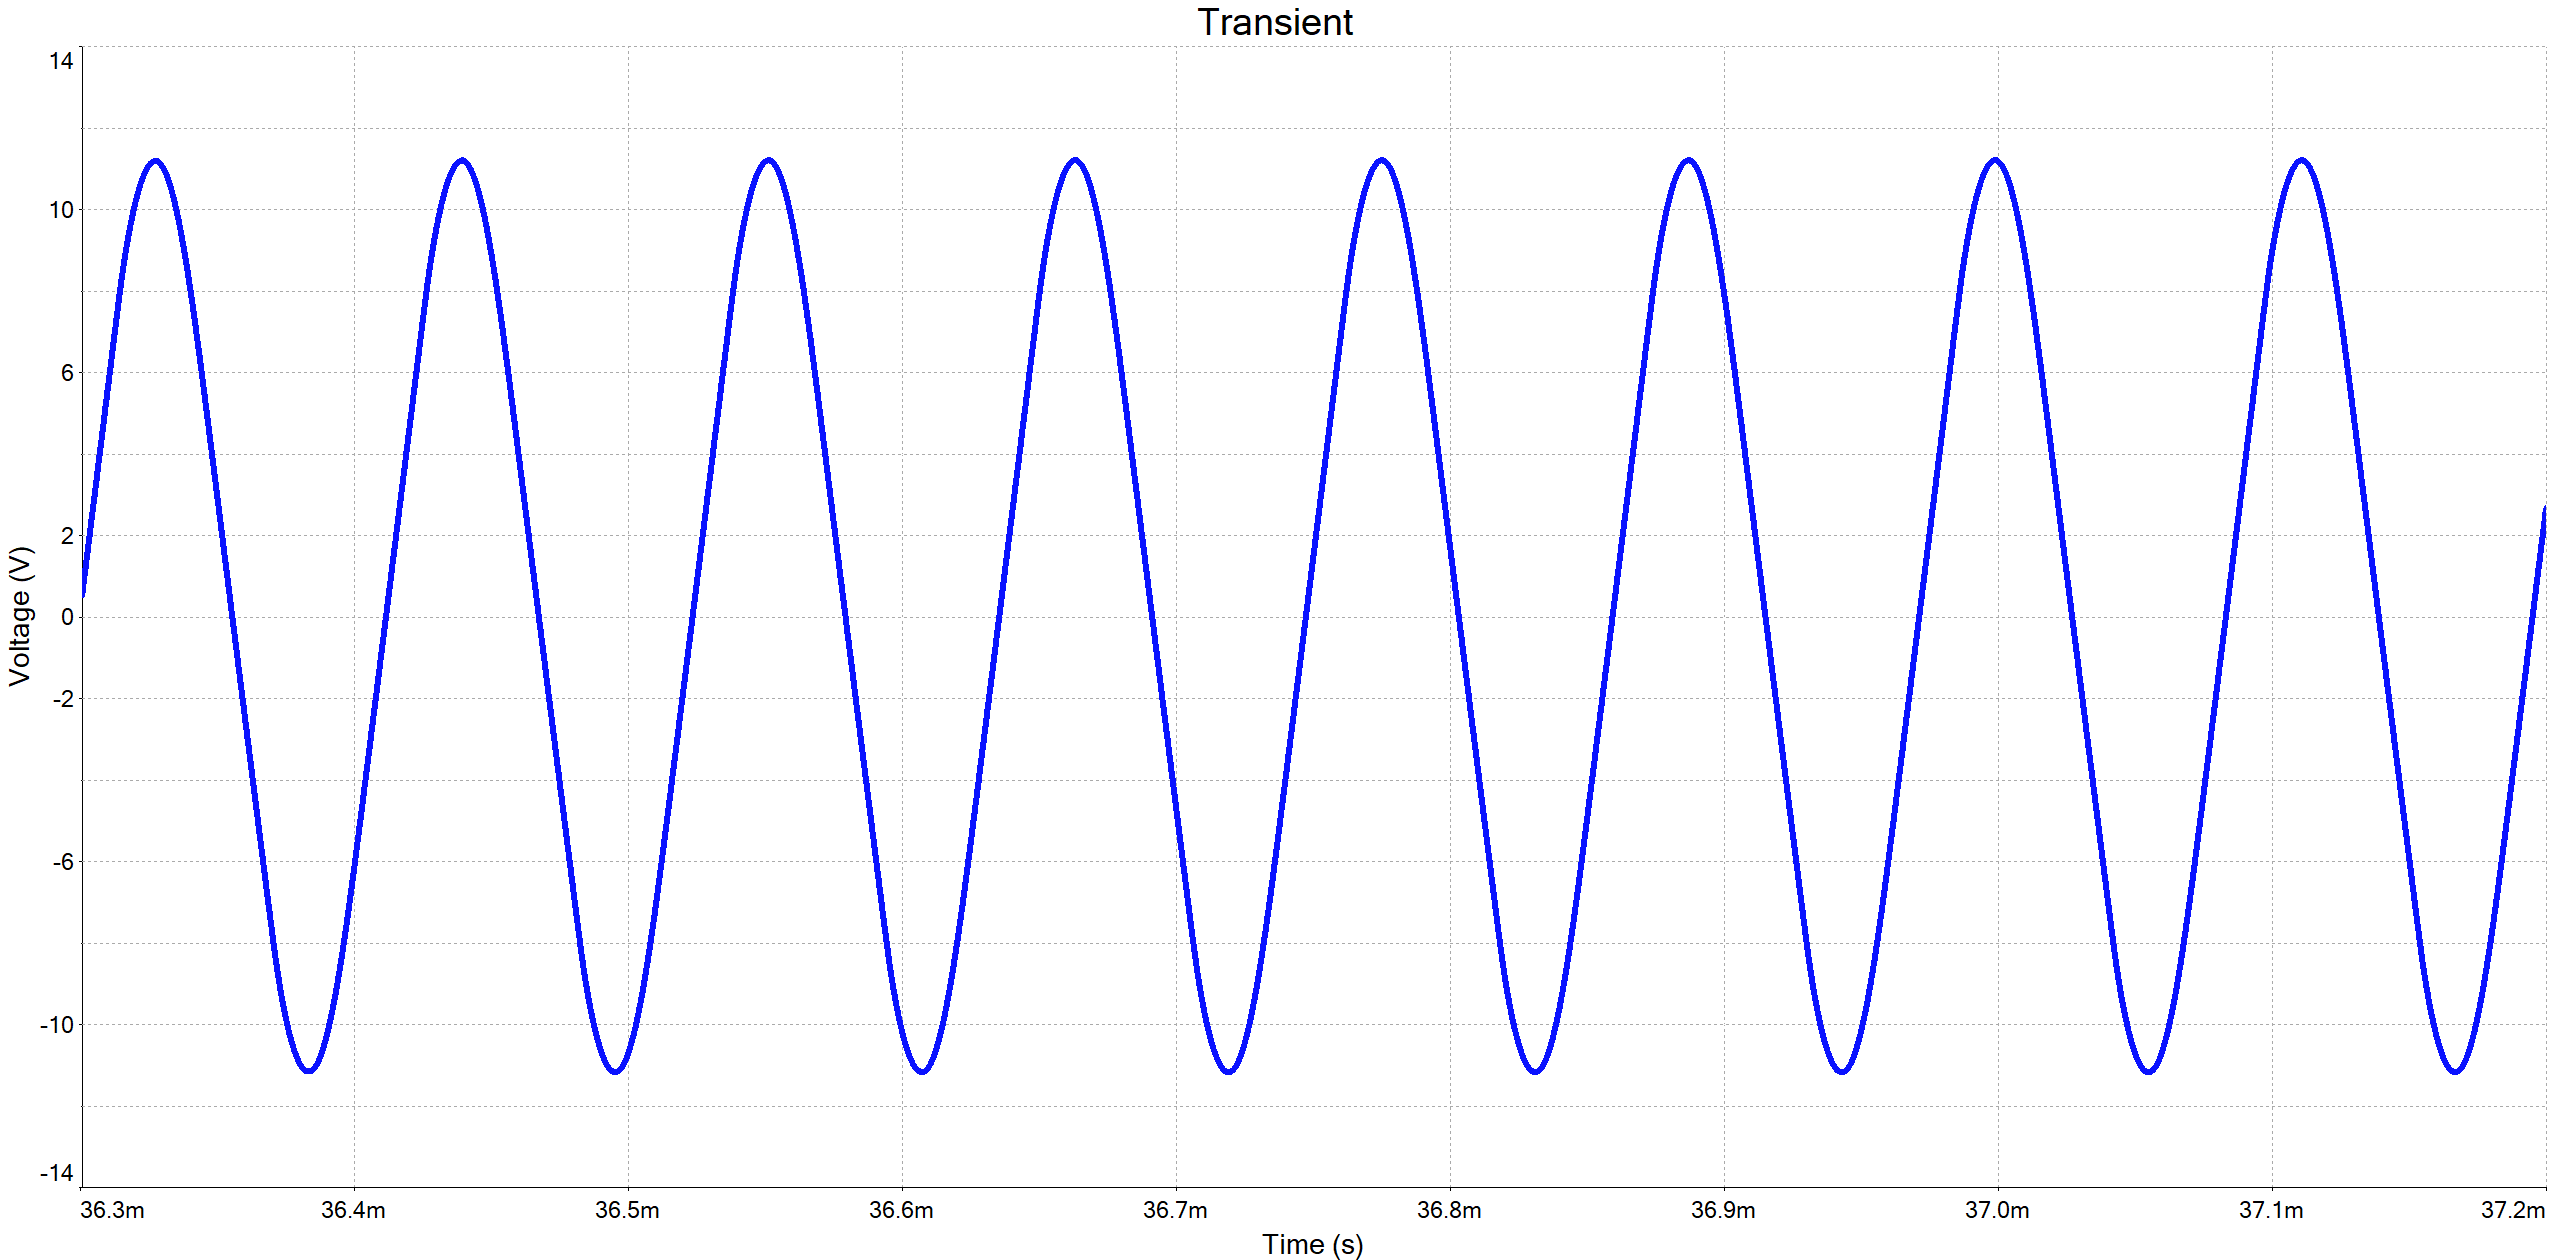
\includegraphics[height=0.32\textwidth]{Images/partatransient.png}\\
    \caption{Oscillating Output}
    \label{fig:oscillatingoutput}
\end{figure}
\FloatBarrier
Using the cursors and measuring the differences between the crests of the plot, we find that the oscillating frequency is 
\boxed{f_o = 8.93kHz}.
Below is the root locus plot:

\begin{figure}
\centering
\begin{minipage}{.5\textwidth}
    \centering
    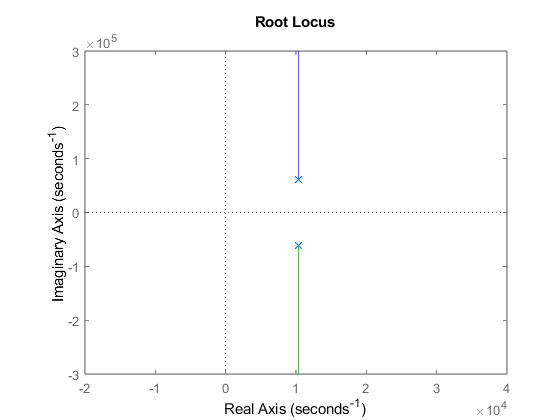
\includegraphics[height=0.7\textwidth]{Images/unstablerootlocus.png}\\
    \caption{Unstable Root Locus Plot}
    \label{fig:unstablerootlocus}
\end{minipage}%
\begin{minipage}{.5\textwidth}
    \centering
    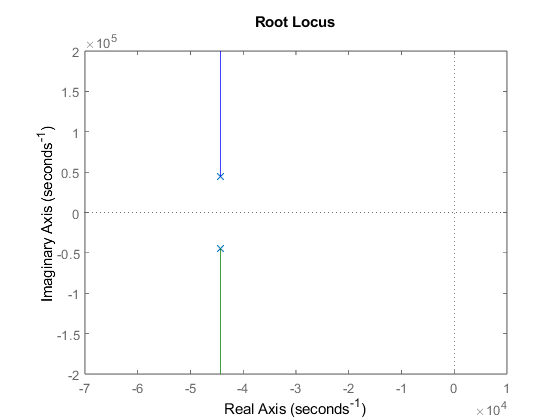
\includegraphics[height=0.7\textwidth]{Images/stablerootlocus.png}\\
    \caption{Stable Root Locus Plot}
    \label{fig:rootlocus}
\end{minipage}
\end{figure}
\FloatBarrier
The root locus plot where $A_M>3$ and $A_M<3$ is Figure \ref{fig:unstablerootlocus} and Figure \ref{fig:rootlocus} respectively. 
We can see from the plot that when the oscillations occour, $A_M$ is greater than 3. This would then cause the system to be 
unstable as shown in Figure \ref{fig:unstablerootlocus}, since the poles are on the right side on the $jw$ axis. When the
poles are on the other side of the $jw$ axis, the system is stable, and doesn't cause the output to oscillate. This happens
when $A_M<3$. The reason why it has to be less than 3 for the system to be stable is because of the characteristic equation in the transfer function. 
If $A_M$ is equal or greater than 3, it causes one of the coefficients in the characteristic equation to be negative, causing instability
in the system and thus, the oscillations occour.

\section{Part B}
Below is our phase shift oscillator circuit:
\begin{figure}[H]
    \centering
    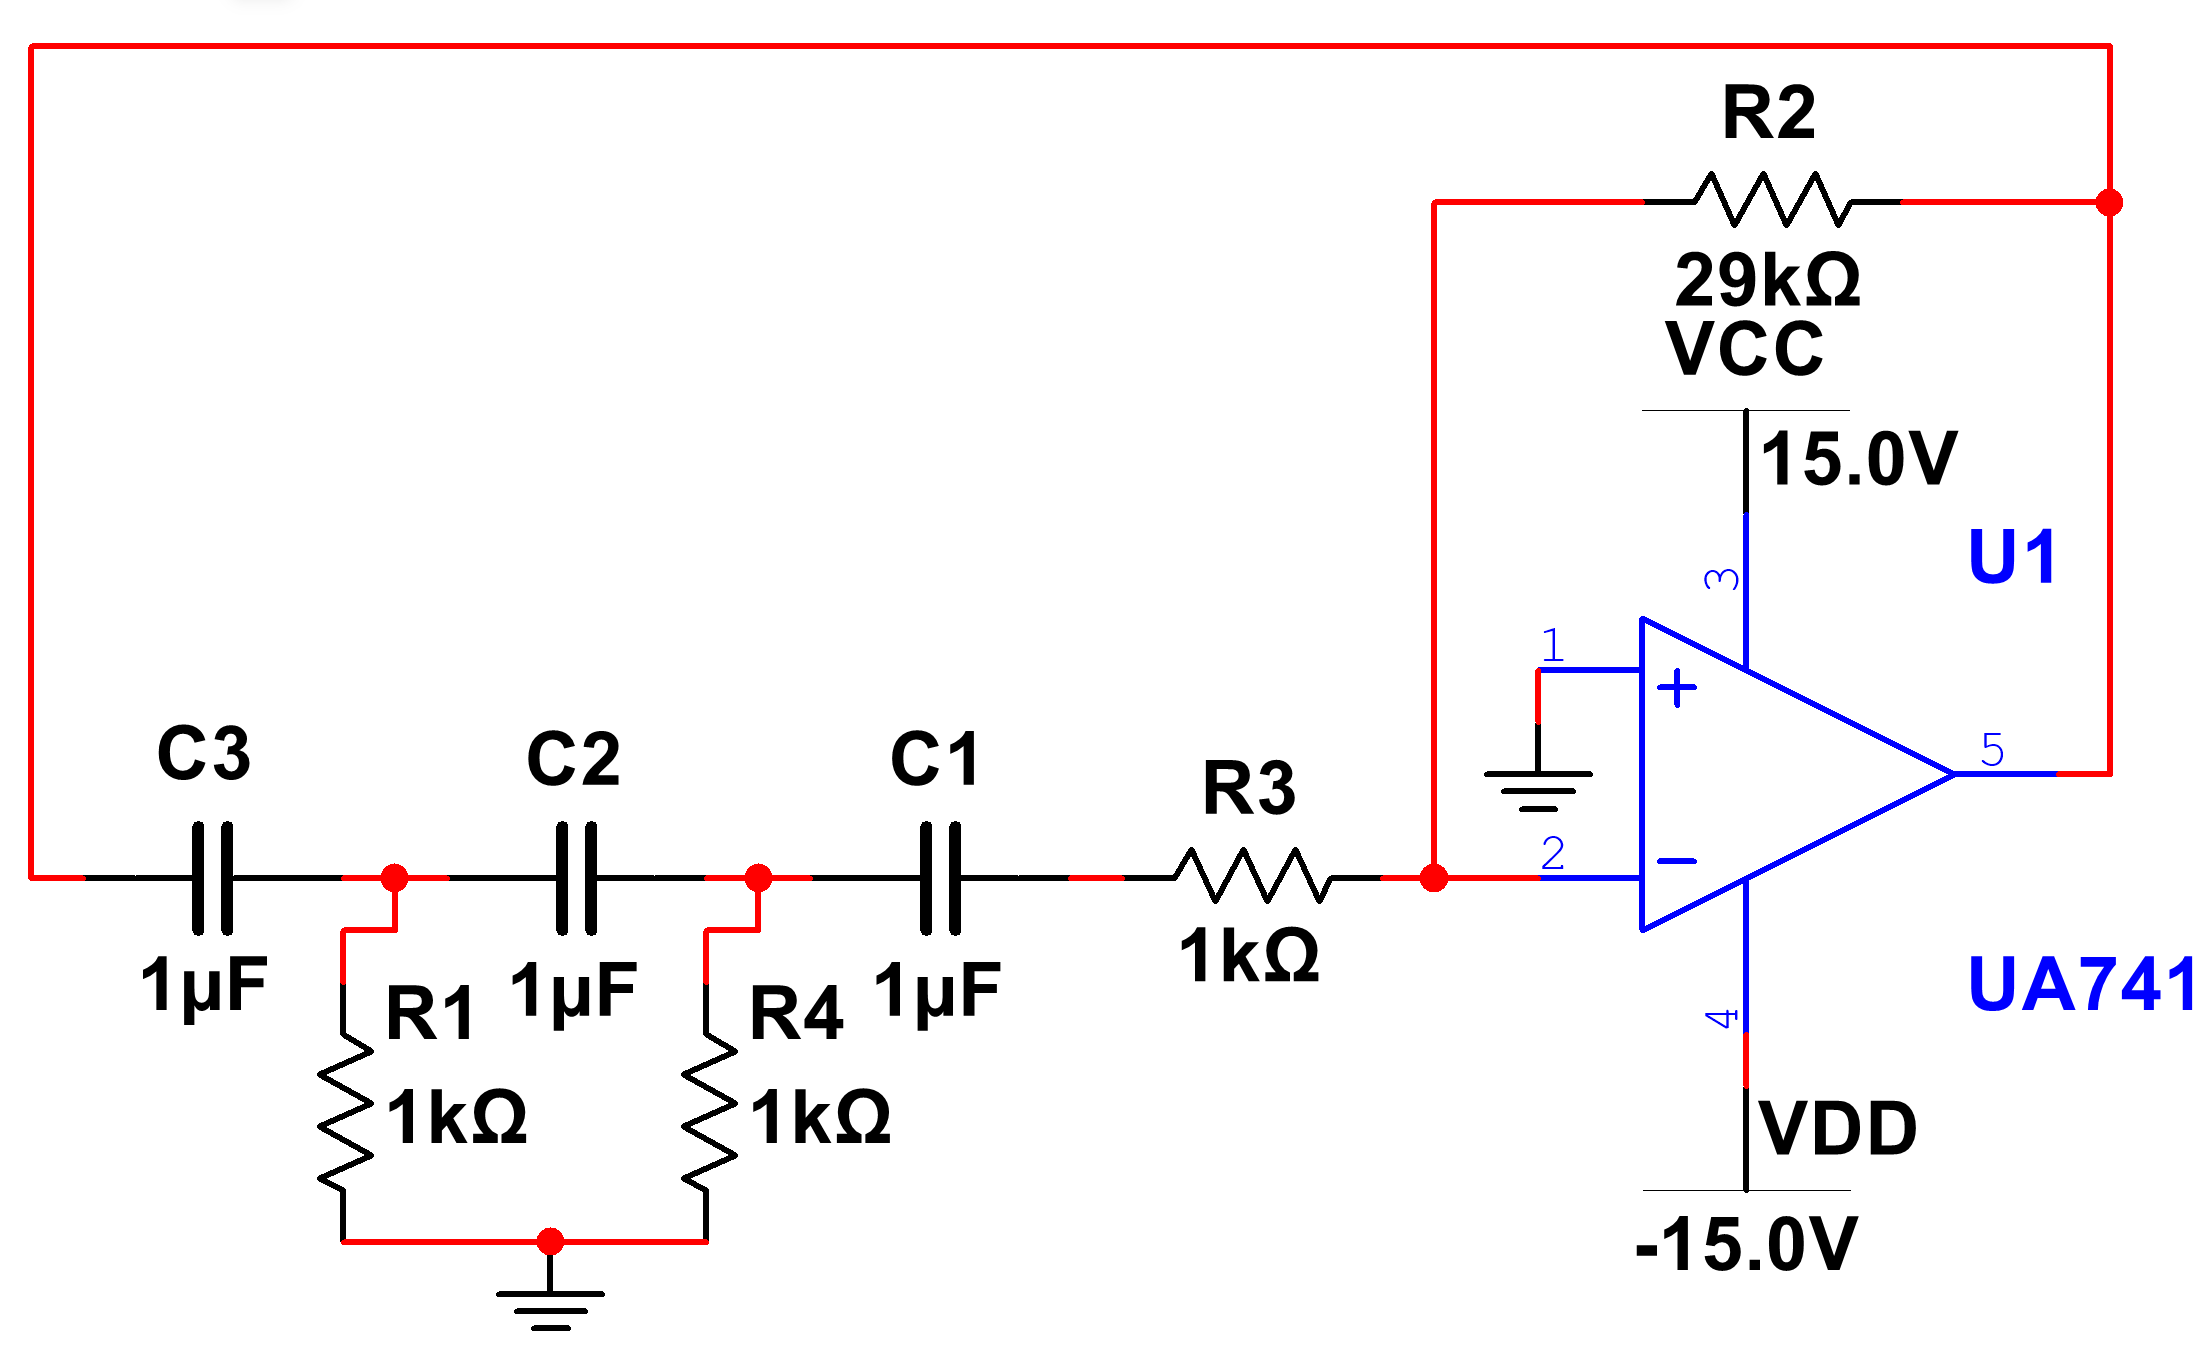
\includegraphics[height=0.2\textwidth]{Images/phaseoscillatorcircuit.png}\\
    \caption{Phase Shift Oscillator Circuit}
    \label{fig:oscillatorcircuit}
\end{figure}
\FloatBarrier

To find the proper value of the 29R resistor, we will simulate the output response for a very large amount of time (in this case, 1000 seconds
was used). Simulating with just $29k\Omega$ we find that the output amplitude eventually decays to zero. Increasing the resistor
to $29.1k\Omega$ makes the output amplitude to be sustained indefinitely. 

Plotting the output of the circuit with the values given in the project document [2] and the increased 29R resistor , we find that 
the output oscillates as shown: 

\begin{figure}[H]
    \centering
    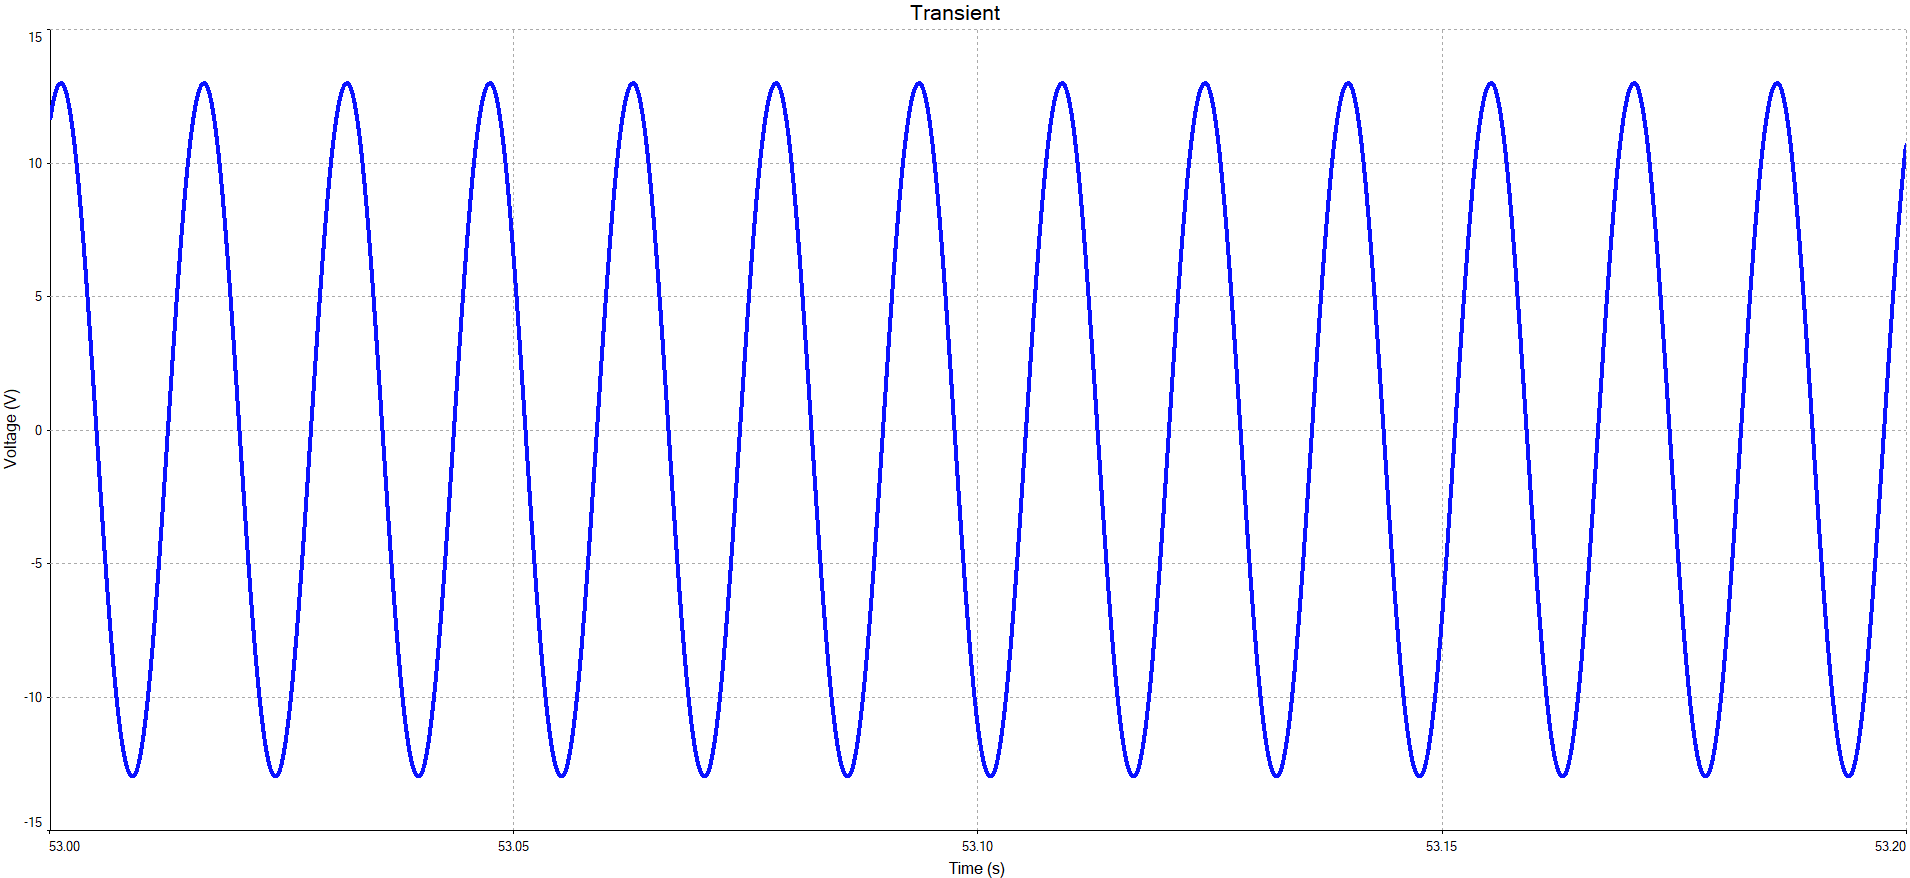
\includegraphics[height=0.3\textwidth]{Images/partbtransient1x.png}\\
    \caption{Circuit Output With Unchanged Circuit Elements}
    \label{fig:oscillatorcircuit1x}
\end{figure}

\begin{figure}[H]
    \centering
    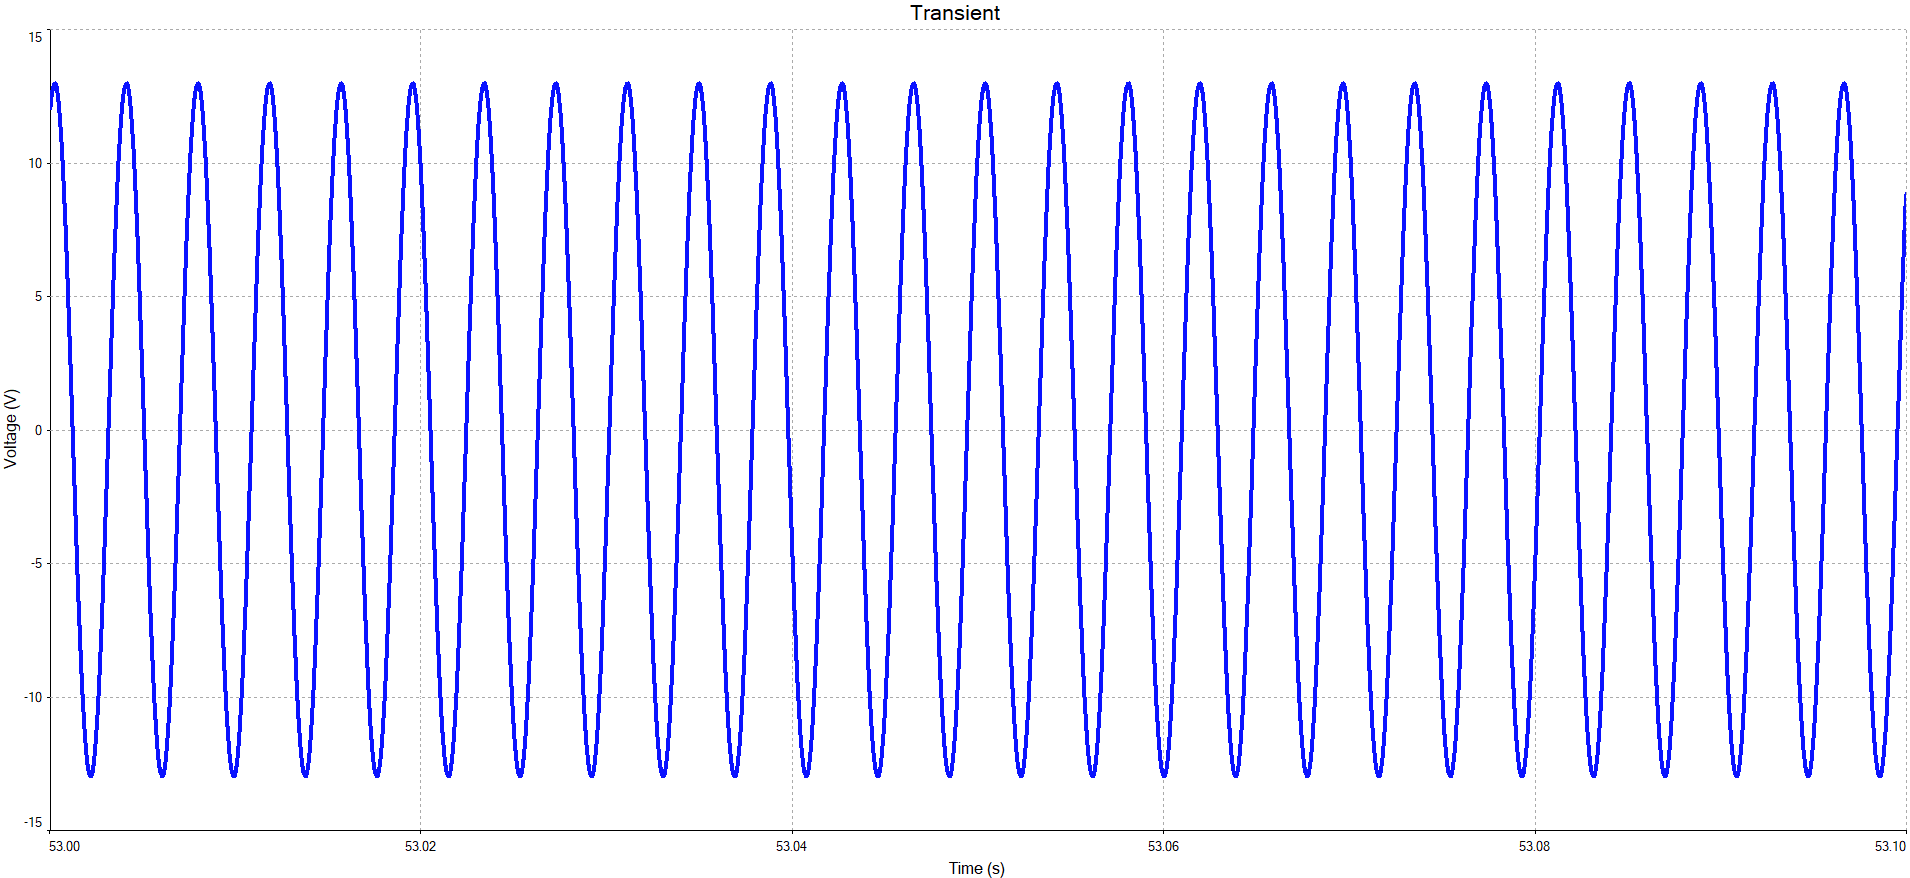
\includegraphics[height=0.3\textwidth]{Images/partbtransient0.5x.png}\\
    \caption{Circuit Output With Half Circuit Elements}
    \label{fig:oscillatorcircuit1x}
\end{figure}

\begin{figure}[H]
    \centering
    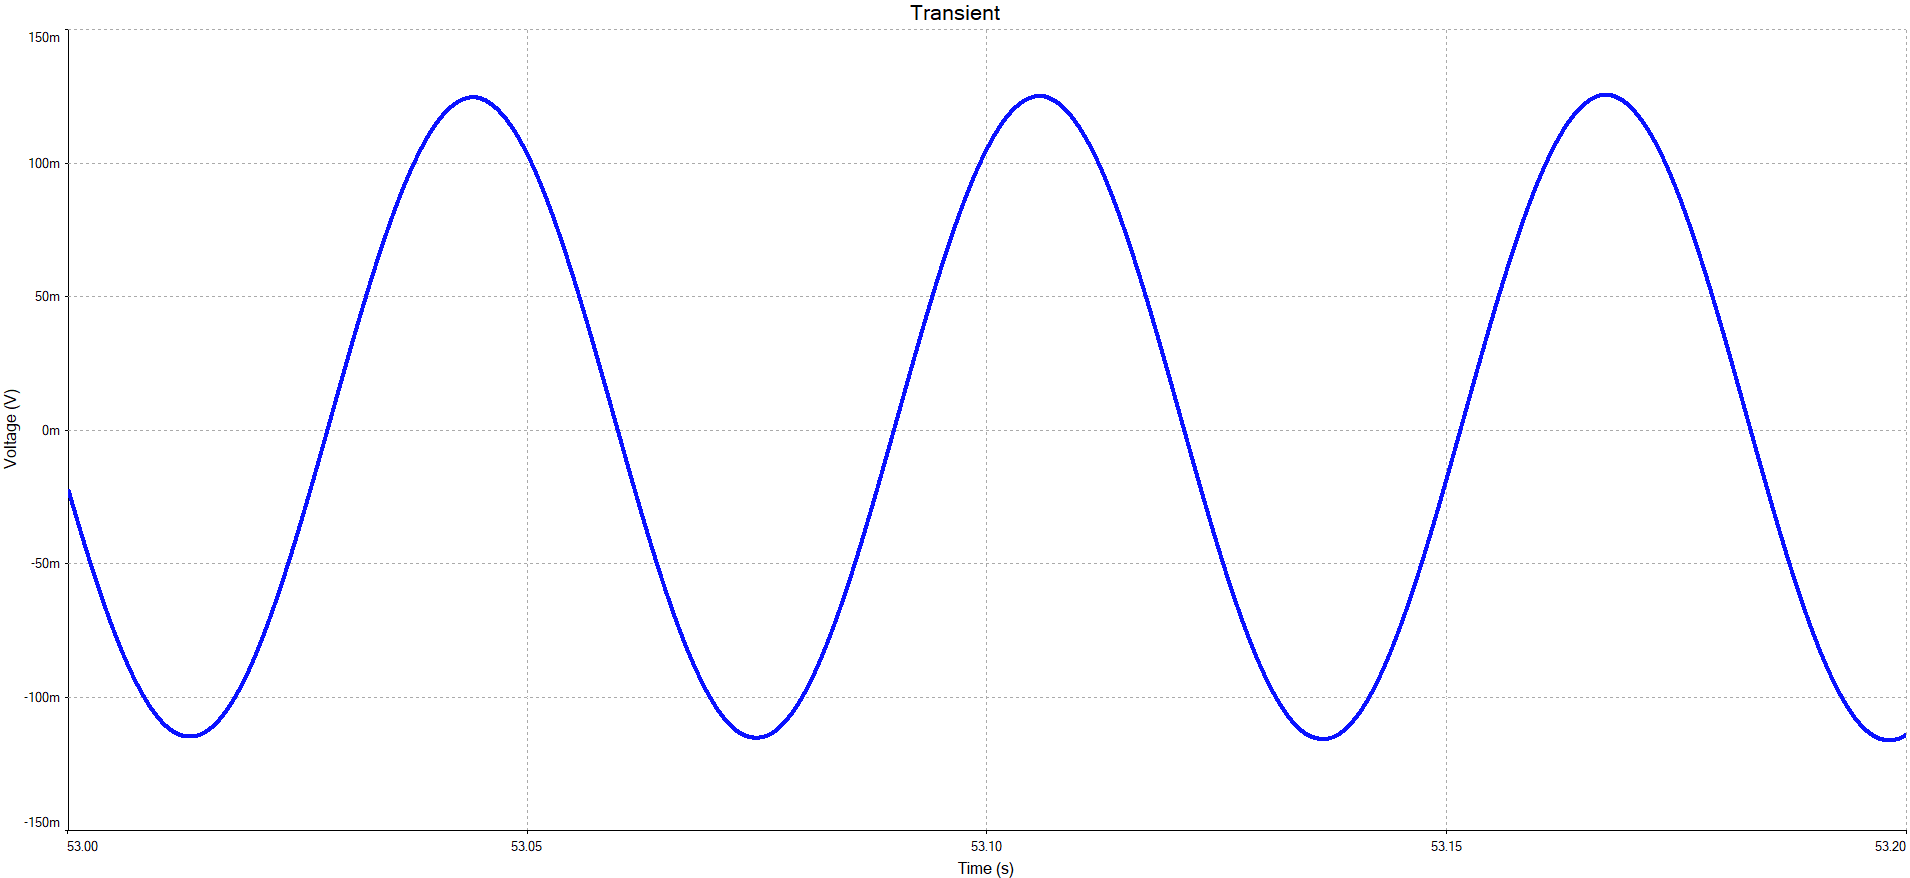
\includegraphics[height=0.3\textwidth]{Images/partbtransient2x.png}\\
    \caption{Circuit Output With Double Circuit Elements}
    \label{fig:oscillatorcircuit1x}
\end{figure}
From class notes[1], we can calculate the output frequency with:
\begin{flalign}
    &f=\frac{1}{2\pi RC \sqrt{6}} \nonumber
\end{flalign} 

Comparing the calculated and measured frequencies for each modified circuit:

\begin{table}[]
    \centering
    \resizebox{0.5\textwidth}{!}{%
    \begin{tabular}{l|l|l|l}
    
    R and C Multiplier & 0.5x & 1x & 2x \\ \cline{1-4}
    Calculated $f_o(Hz)$ & 259.899 & 64.975 & 16.244 \\ \cline{1-4}
    Measured $f_o(Hz)$ & 259.067 & 64.872 & 16.221 \\ \cline{1-4}
    \% Error & 0.32 & 0.15 & 0.14
    \end{tabular}%
    }
    \caption{Calculated and Measured Frequencies}
    \label{CalculatedMeasuredFrequencies}
\end{table}
\FloatBarrier
We can observe that the calculated and measured values are very close to each other.

\section{Part C}
Below is our Feedback Circuit:
\begin{figure}[H]
    \centering
    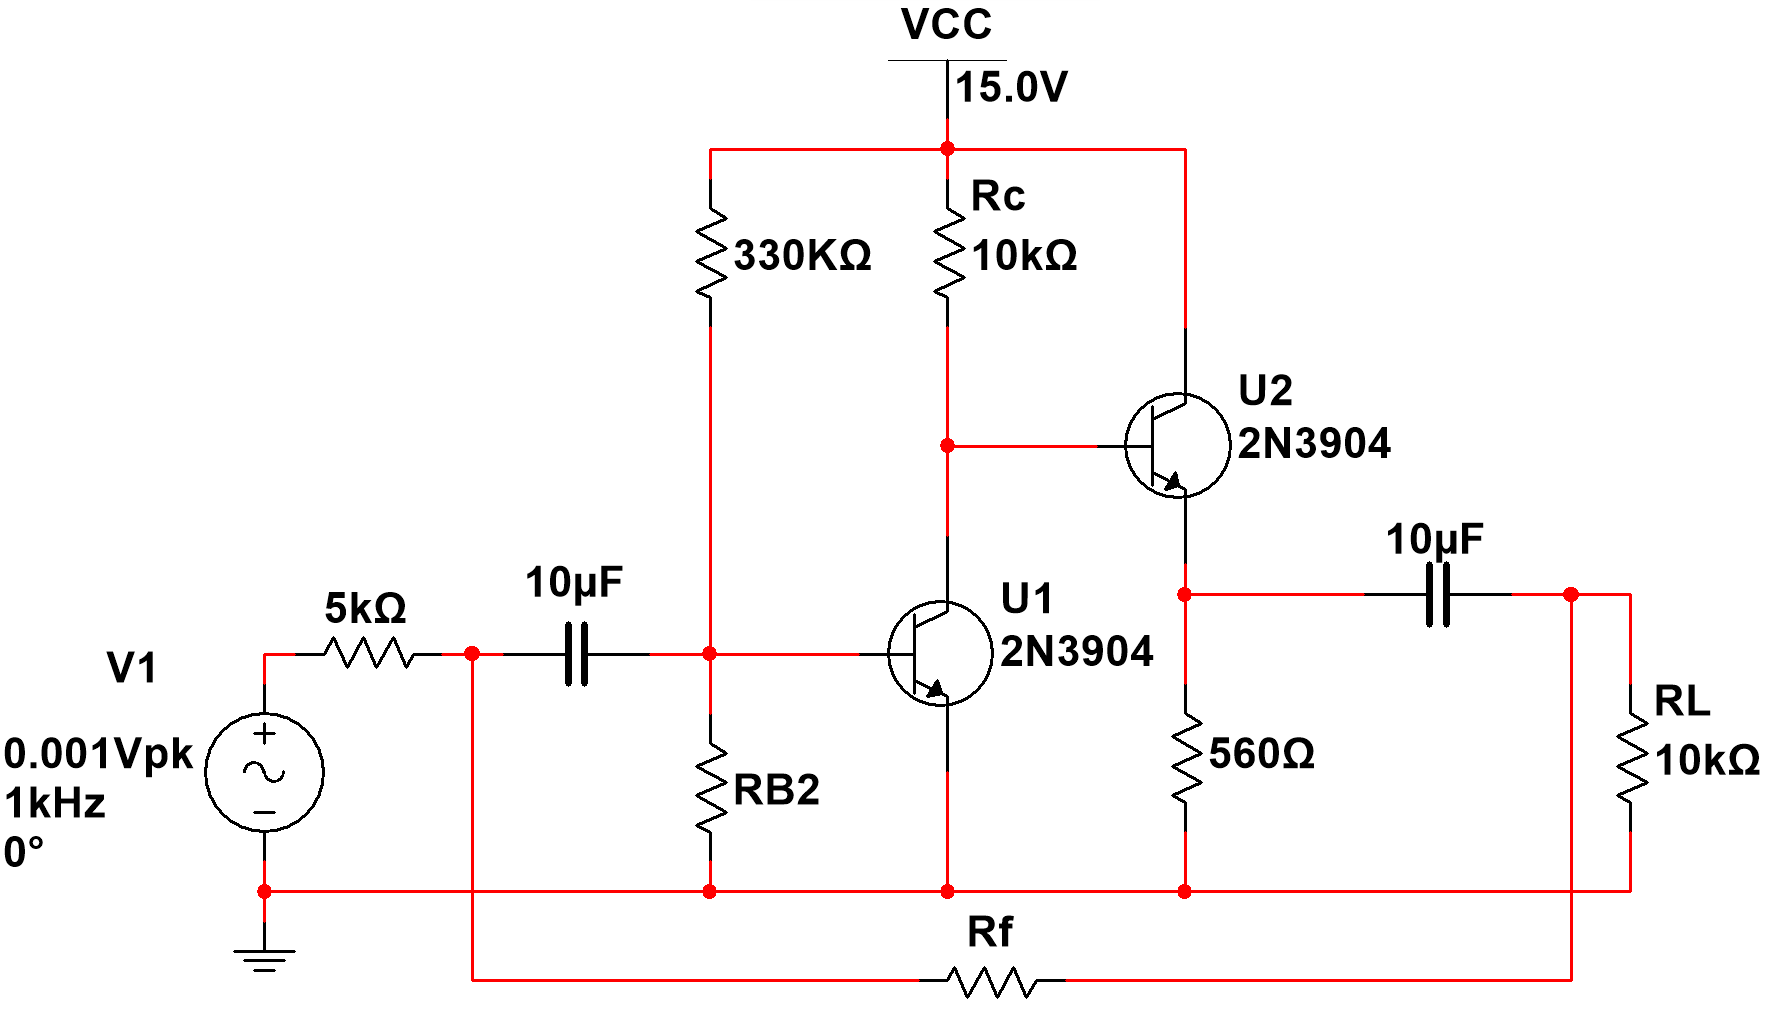
\includegraphics[height=0.25\textwidth]{Images/partCcircuit.png}\\
    \caption{Feedback Circuit}
    \label{fig:feedbackcircuit}
\end{figure}

Since we want to find the value of $R_{B2}$ that creates the largest open-loop gain at 1kHz, we will be setting our
input voltage at 1kHz at 1mV. To find the value, we will be doing a parameter sweep with a transient response to 
find which resistance value results in the largest gain. We find that after doing the parameter sweep,
the value $R_{B2}$ to be around \boxed{20k\Omega}. Resistance values above $20k\Omega$
, we find that the output amplitude decreases. The paramater sweep is shown below:

\begin{figure}[h!]
    \centering
    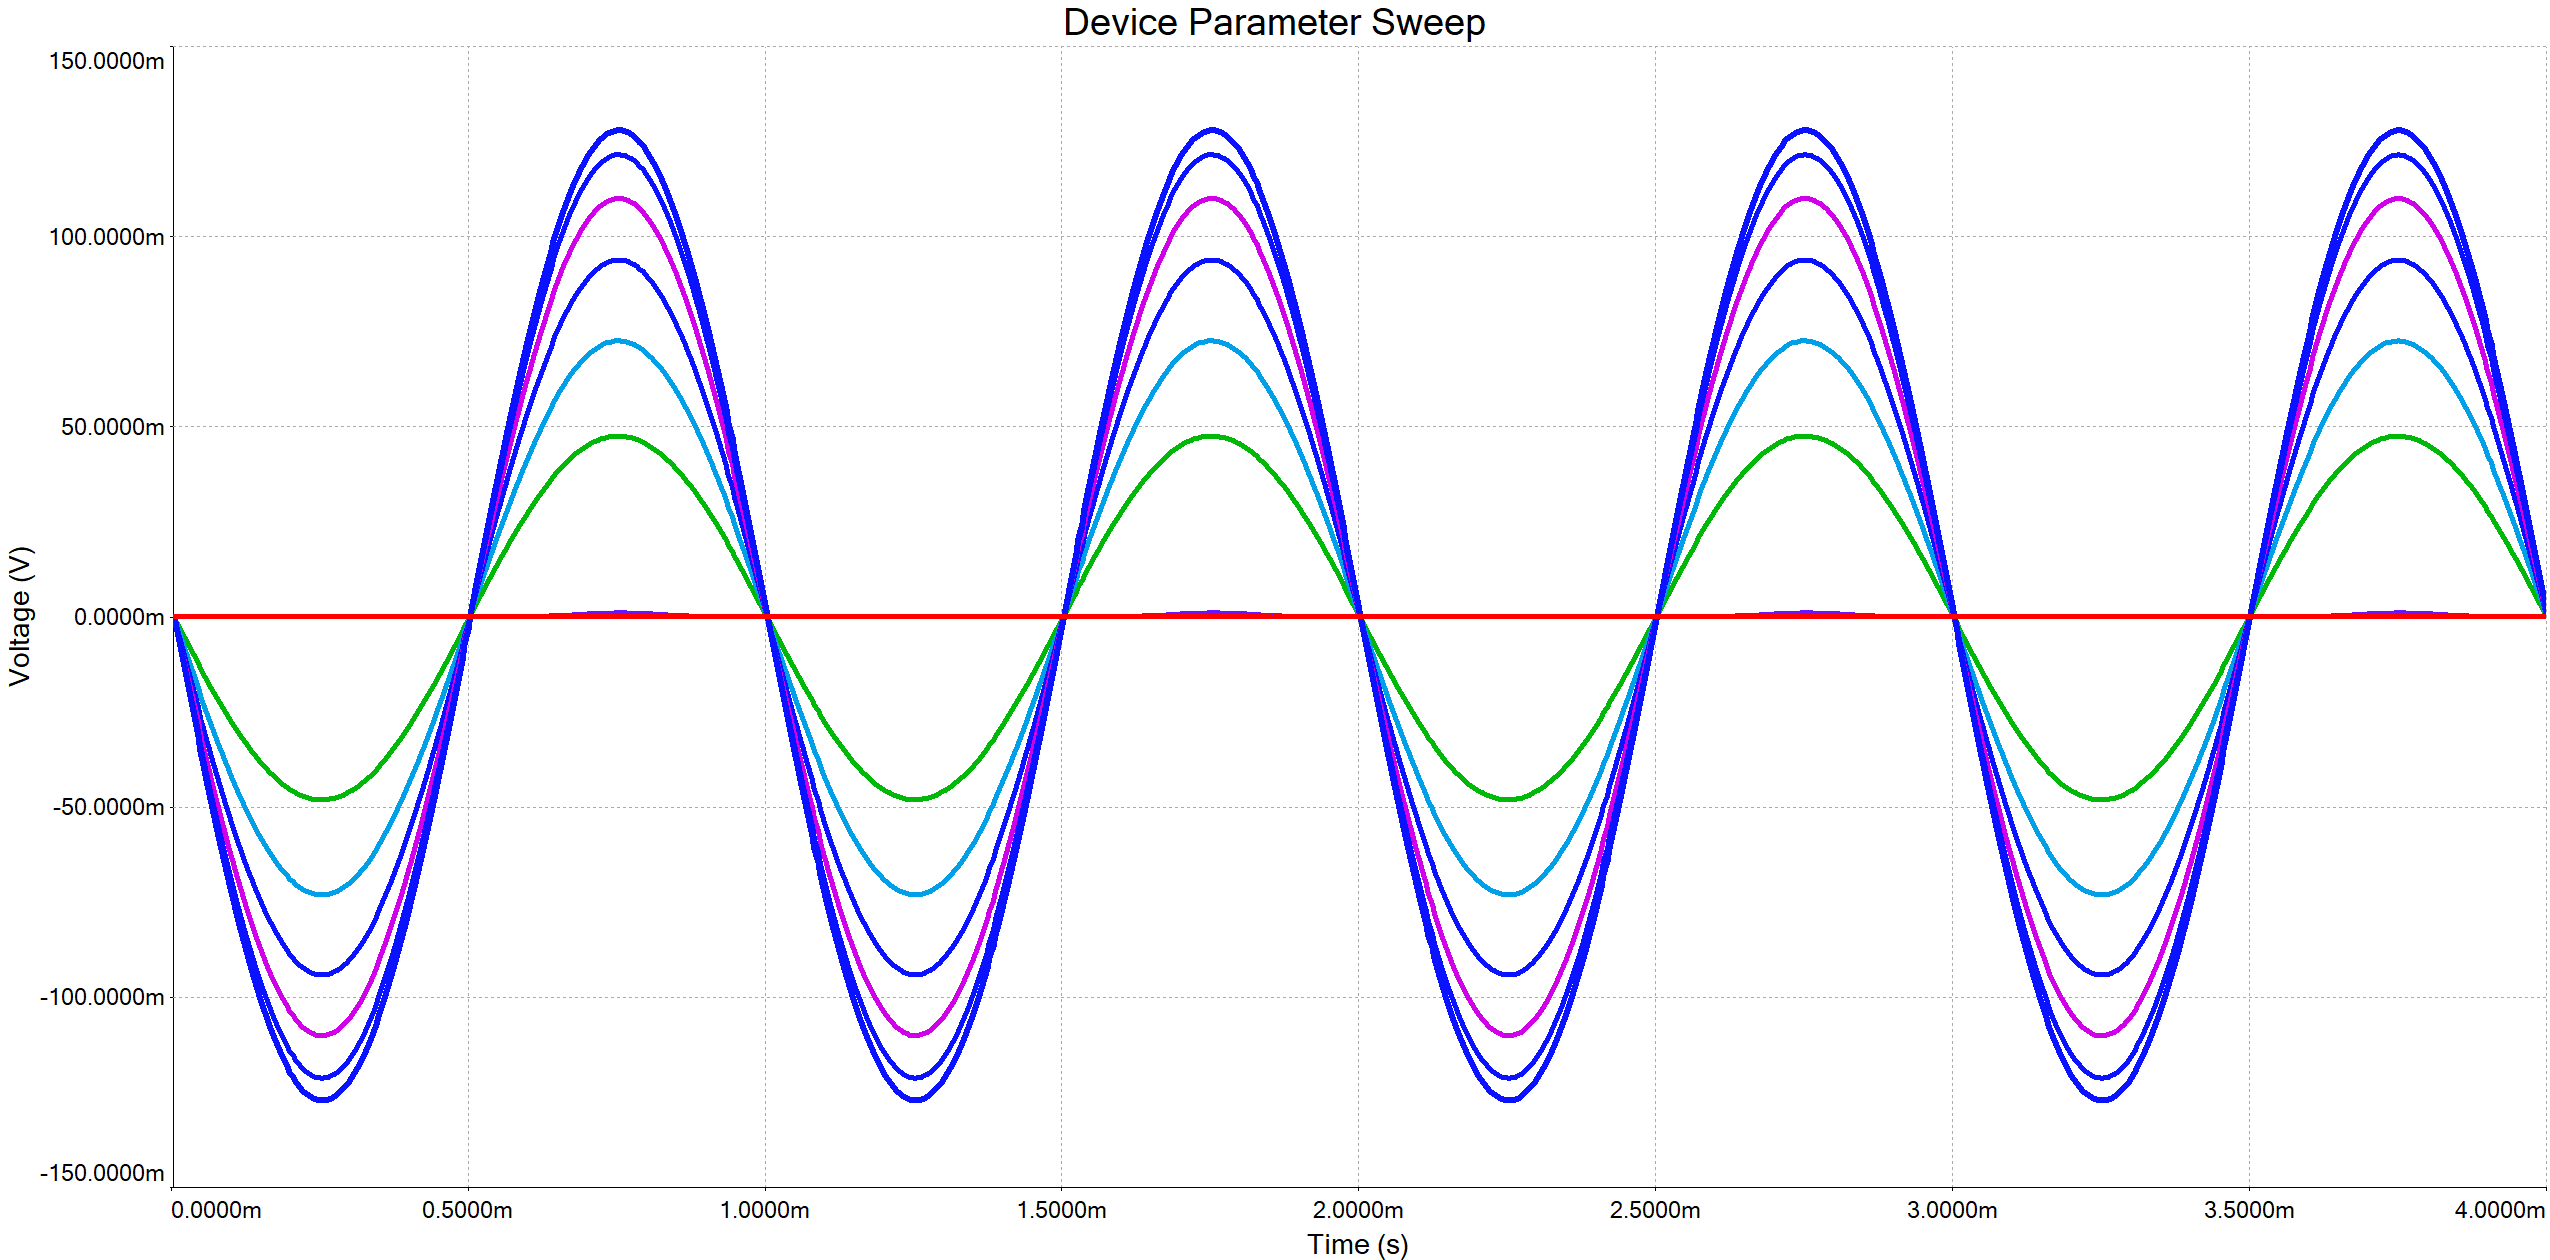
\includegraphics[height=0.4\textwidth]{Images/parametersweep.png}\\
    \caption{Parameter Sweep with $R_{B2}$ and Transient Response}
    \label{fig:parametersweep}
\end{figure}


\subsection{Part 1}
To measure the DC Operating points, we will be using the DC Circuit below:
\begin{figure}[h!]
    \centering
    \includegraphics[height=0.25\textwidth]{Images/partCDC.png}\\
    \caption{Feedback DC Circuit}
    \label{fig:feedbacdccircuit}
\end{figure}
\FloatBarrier
For this project, we will be assuming that $V_T$= 0.025V. We can use these formulas to 
calculate our transistor parameters:
\begin{center}
    $r_\pi= \frac{V_T}{I_B}$ ,$\beta = \frac{I_C}{I_B}$ and $g_m = \frac{\beta}{r_\pi}$
\end{center}
Here are the DC Operating points, with our measured $r_\pi,g_m$, and $h_{FE}$:
\FloatBarrier
\begin{table}[h!]
    \centering
    \begin{tabular}{l|lllllllll}
     & $I_C$ & $I_B$ & $I_E$ & $V_C$ & $V_B$ & $V_E$ & $g_m$ & $r_\pi$ & $h_{FE}$ \\ \cline{1-10}
    Q1 & 1.29mA & 10.8uA & 1.31mA & 1.90V & 0.654V & 0V & 0.05 & 2.315k$\Omega$ & 119  \\ \cline{1-10}
    Q2 & 2.19mA & 15.4uA & 2.21mA & 15V & 1.90V & 1.23V & 0.09 & 1.623k$\Omega$ & 142
    \end{tabular}%
    \caption{DC Operating Points}
    \label{DC Operating Points}
\end{table}

\subsection{Part 2}
Here is the open loop frequency response plot:
\begin{figure}[h!]
    \centering
    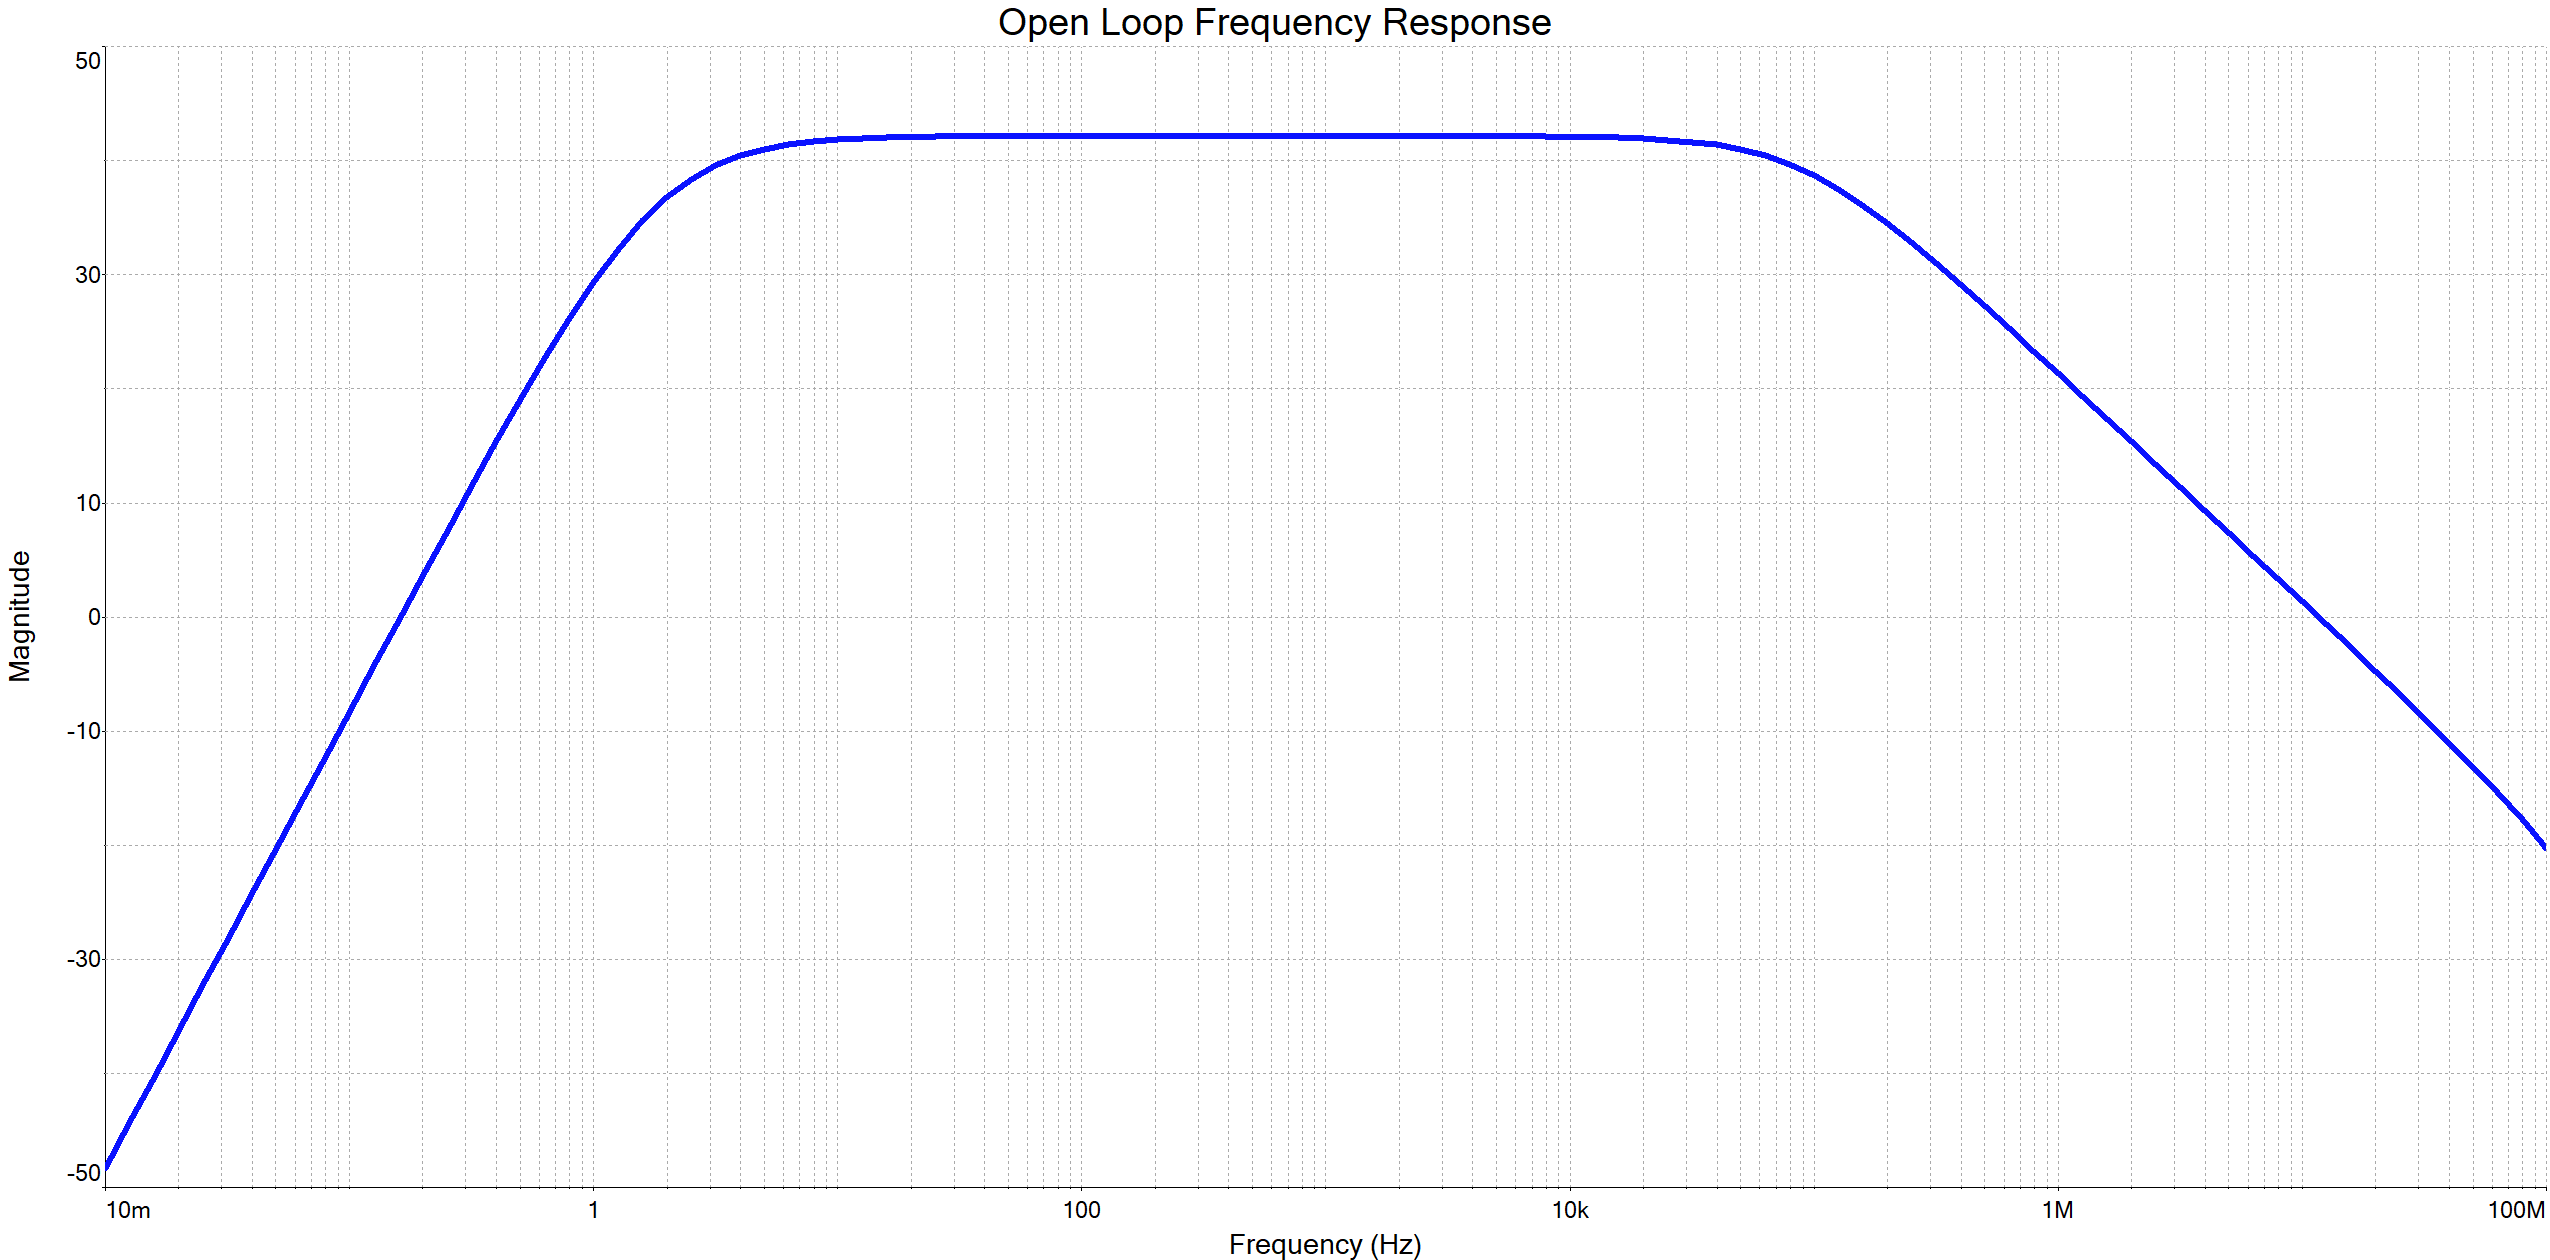
\includegraphics[height=0.39\textwidth]{Images/partCbode.png}\\
    \caption{Open Loop Frequency Response}
    \label{fig:olfreqresponse}
\end{figure}
Measuring with the cursors in our simulation software, we find that the 
3dB points are: 
\begin{center}
    \boxed{w_{L3dB} = 2.9219 *2\pi [\frac{rad}{s}], w_{H3dB} = 91.3083*2\pi*10^3[\frac{rad}{s}] } 
\end{center}
We can also find our mid-band gain \boxed{A_m = 127.557\frac{V}{V}}.
In order to find the input and output resistance at 1kHz, we will be measuring the voltage 
and current at the input and output. We will measure the short circuit current and open circuit 
voltage for the output impedance. After measuring, we find: 
\begin{center}
$R_{in} = \frac{240\mu V}{93.4nA}$ = \boxed{2.569k\Omega}, 
$R_{out} = \frac{1.24V}{1.39mA} = $ \boxed{892.1\Omega}
\end{center}









\newpage
\section{Appendix}
\begin{flalign}
    &k = 3 - \sqrt(2)\\
\end{flalign}
\section{References}
1. ELEC 301 Class notes 
\newline
2. Mini Project 4 Document
\newline
3. Standard Resistor and Capacitor Values (Canvas)
\newline
4. Circuit Maker SPICE Model


\end{document}